\documentclass[12pt]{article}\usepackage[]{graphicx}\usepackage[]{color}
\usepackage[top=1in,left=1in, right = 1in, footskip=1in]{geometry}

\title{A note on observation processes in epidemic models}
\author{Sang Woo Park and Benjamin M. Bolker}

\usepackage{tabularx}

\usepackage{amsmath}
\usepackage{natbib}
\usepackage{hyperref}
\bibliographystyle{chicago}
\date{\today}

\usepackage{bm}

\usepackage{afterpage}
\usepackage{pdflscape}

\newcommand{\etal}{\textit{et al.}}

\newcommand{\comment}[3]{\textcolor{#1}{\textbf{[#2: }\textit{#3}\textbf{]}}}
\newcommand{\bmb}[1]{\comment{cyan}{BMB}{#1}}
\newcommand{\swp}[1]{\comment{magenta}{SWP}{#1}}
\newcommand{\citetapos}[1]{\citeauthor{#1}'s \citeyearpar{#1}}

\newcommand{\fref}[1]{Fig.~\ref{fig:#1}}
\begin{document}

\maketitle

\section*{Abstract}

Many disease models focus on characterizing
the underlying transmission mechanism but make simple, possibly naive assumptions about
how infections are reported. In this note, we use a simple deterministic
Susceptible-Infected-Removed (SIR) model to compare two common assumptions 
about disease incidence reports: individuals can report their infection as soon as
they become infected or as soon as they recover. We show that
incorrect assumptions about the underlying observation processes can bias
estimates of the basic reproduction number and lead to overly
narrow confidence intervals.

\section{Introduction}

Mechanistic analyses of epidemic time series allow us to make inference about the underlying 
transmission mechanisms, estimate biologically relevant parameters, and 
predict the course of an outbreak \citep{breto2009time}. In order to make 
precise and accurate inferences, disease modelers have sought to build
more realistic process models. For example, the time series of reported
measles cases from London in the prevaccination era has been analyzed many times, using
variety of models accounting for time-varying transmission rates \citep{fine1982measles}, 
realistic age structure \citep{schenzle1984age},
metapopulation structure \citep{xia2004measles}, continuous-time infection processes 
\citep{cauchemez2008likelihood}, and extra-demographic variability \citep{he2009plug}. 

Despite the amount of effort put into developing better process models, 
disease modelers often neglect details of the observation processes associated with
new disease case reports (often referred to as incidence time series).
Many disease models effectively assume that new cases are reported
instantaneously when an individual is infected (e.g., \cite{martinez2016differential, 
kennedy2018modeling, pons2018serotype}) or when an individual becomes symptomatic
(e.g., \cite{bhadra2011malaria, king2015avoidable}); 
some models (e.g., \cite{breto2009time, he2009plug, lin2016seasonality})
assume that infections are counted upon recovery (because diagnosed cases
are controlled and are effectively no longer infectious). 
\bmb{Maybe mention King et al. -- completely ignored observation processes}

Note that incidence (the number of \emph{newly} infected individuals) is different from 
prevalence (the number of \emph{currently} infected individuals) \citep{bjornstad2018epidemics};
the observed dynamics of incidence depend on the reporting time step (because the sum of 
true incidence is equal to the final size of an epidemic), whereas those of
prevalence do not. 
While they are relatively
uncommon, some models do not make a clear distinction between prevalence and 
incidence 
\citep{capistran2009parameter, hooker2010parameterizing, yang2013stability, gonzalez2014fractional}.

Here, we use a simple Susceptible-Infected-Removed (SIR) model to study how 
assumptions about the underlying observation processes affect parameter estimates
of the SIR model. We show that making wrong assumptions about the timing of 
incidence reports can lead to biased parameter estimates and overly narrow 
confidence intervals. 

\section{Methods}

The Susceptible-Infected-Removed (SIR) model describes how a disease spreads in a
homogeneous population:
\begin{equation}
\begin{aligned}
\frac{dS}{dt} &= - \beta S \frac{I}{N}\\
\frac{dI}{dt} &= \beta S \frac{I}{N} - \gamma I\\
\frac{dR}{dt} &= \gamma I,
\end{aligned}
\end{equation}
where $\beta$ is the contact rate per unit time, $\gamma$ is the recovery rate per unit time, 
and $N = S + I + R$ is the total population size. 
We define incidence at time $t$ as the number of newly infected
individuals that are infected between time $t- \Delta t$ and time $t$, where $\Delta t$ is
the reporting time step. We expect infected cases to be reported some time after infection;
the number of reported cases during a time period defines the \emph{observed} incidence. 

For brevity, we consider two extreme cases: individuals instantaneously report
their infection when they become infected or when they recover. The observed incidence 
measured upon infection, $i_1(t)$, can be defined by the integral:
\begin{equation}
i_1(t) = \int_{t - \Delta t}^{t} \beta S \frac{I}{N} dt.
\end{equation}
Equivalently, we can keep track of cumulative incidence, $C$, by adding a 
new state variable described by $dC/dt = \beta S I/N$ and taking the difference between 
the two consecutive reporting periods: $i_1(t) = C(t) - C(t-\Delta t)$. Likewise, 
incidence measured upon recovery, $i_2(t)$, can be defined by the integral:
\begin{equation}
i_2(t) = \int_{t-\Delta t}^{t} \gamma I dt,
\end{equation}
or by the consecutive difference in the cumulative number of recovered cases:
$i_2(t) = R(t) - R(t - \Delta t)$.
Finally, we model reporting error using a negative binomial distribution with a
mean of either $\rho i_1(t)$ or $\rho i_2(t)$, where $\rho$ is the reporting rate, and
an over-dispersion parameter $\theta$. For convenience, we will refer to these two
negative binomial models as infection model and recovery model hereafter; 
similarly, we will refer to epidemic time series generated from these
negative binomial models with two different means ($\rho i_1(t)$ and $\rho i_2(t)$)
as infection time series and recovery time series.

In this study, we focus on estimating 5 parameters: the basic reproductive
number $\mathcal R_0 = \beta/\gamma$, mean infectious period $1/\gamma$, 
reporting rate $\rho$, an overdispersion parameter $\theta$, and the initial
proportion of the infected individuals $i_0$. The initial proportion of
susceptible individuals is assumed to be $1 - i_0$. The total population
size $N$ is assumed to be known.

\section{Results}

\begin{figure}[!t]
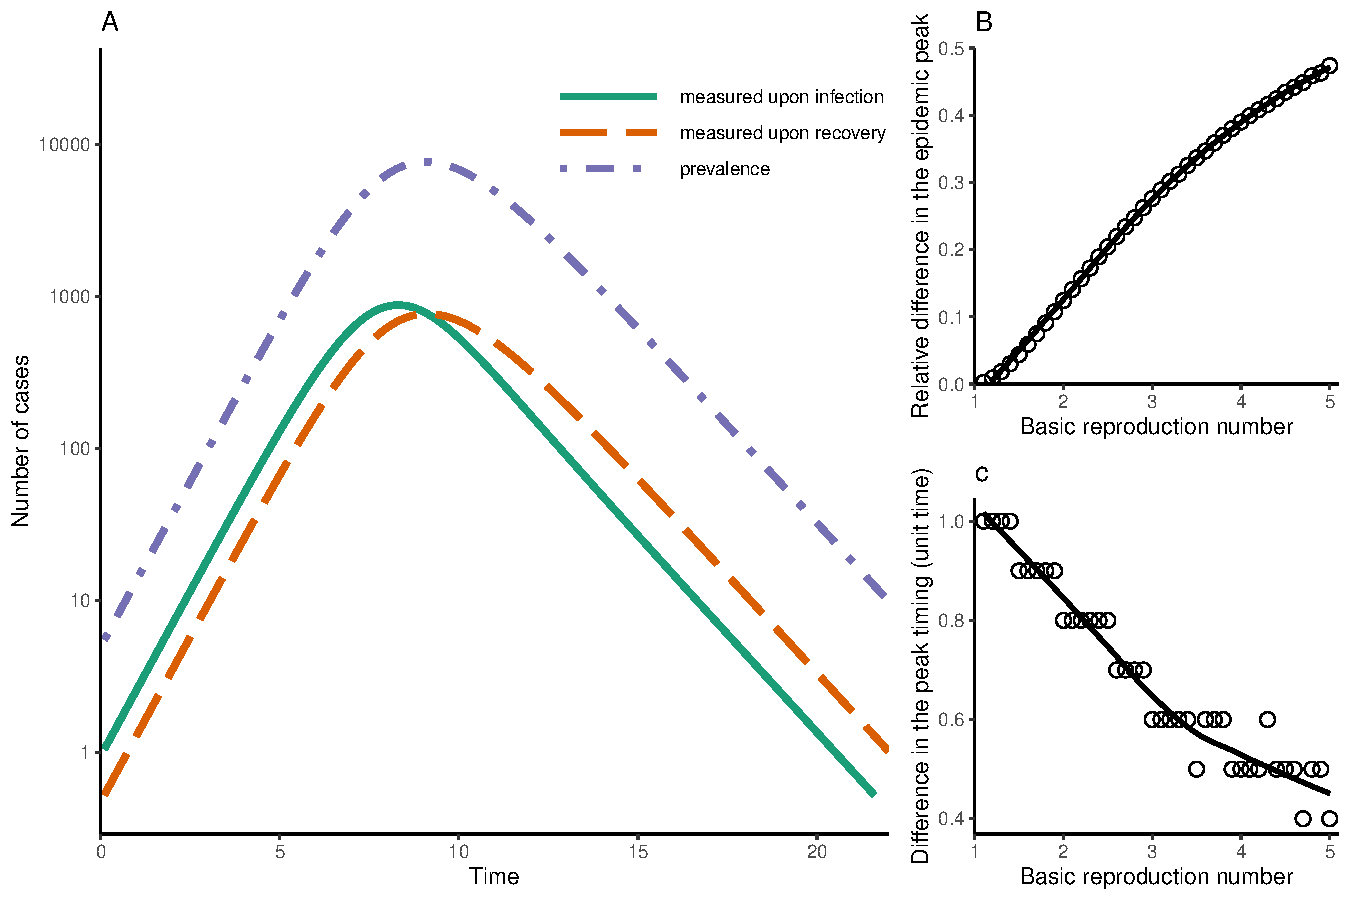
\includegraphics[width=\textwidth]{../figure/example.pdf}
\caption{
\textbf{A comparison of incidence measured at two different time points in infection.}
A deterministic SIR model is simulated using the following parameters: 
$\mathcal R_0 = 2$, $1/\gamma = 1$ time units, $N = 1 \times 10^5$, $i0 = 1 \times 10^{-4}$,
and $\Delta t = 0.1$ time units.
}
\end{figure}

Figure 1 compares the deterministic dynamics of incidence curves,
$i_1(t)$ and $i_2(t)$, and a prevalence curve $I(t)$. A lag in reporting time delays
the observed epidemic peak timing and slightly reduces the size of the peak. However, 
these differences in the reporting time have little effect on the overall shape 
of the epidemic curve. In the presence of observation and process error, we
do not expect to be able to distinguish between the two reporting processes
based on the time series alone (and we rarely know \emph{a priori} the delay distribution between when an individual is infected and when that case is reported).
Therefore, one might naively expect assumptions about the timing of case reporting to have negligible effect on inference.

In order to understand how assumptions about the timing of case reporting affect 
parameter estimates of the SIR model, we simulate observed epidemic time series
(infection time series and recovery time series) 
100 times and fit both infection and recovery models to each 
time series. We compare the estimates of the basic reproductive number $\mathcal R_0$,
and the coverage of our confidence intervals, defined as the proportion of confidence intervals that
contain the true value (95\% confidence interval is expected to contain the true value
95\% of the time by definition). Figure 2 summarizes the results.

When we try to estimate all 5 parameters, fitting the recovery model to
infection time series underestimates the basic reproduction number and 
gives a slightly low coverage (Figure 2A). Fitting the infection model to recovery
time series slightly overestimates the basic reproduction number but gives 
good coverage. Fitting the correct models to their corresponding time series
gives unbiased estimates and good coverage.

\begin{figure}
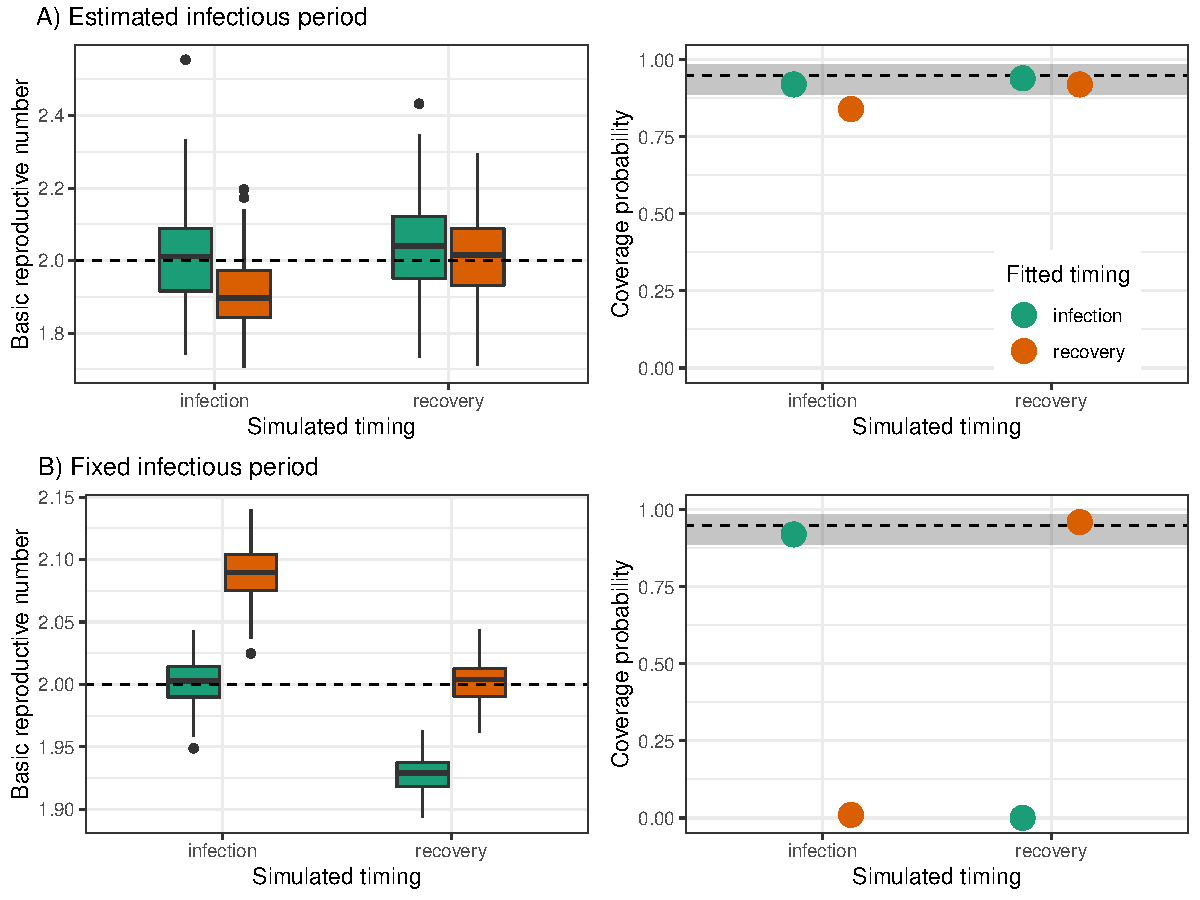
\includegraphics[width=\textwidth]{../figure/compare_deterministic.pdf}
\caption{
\textbf{A comparison of incidence measured at two different time points in infection.}
We simulate infection time series and recovery time series 100 times using the 
following parameters:  
$\mathcal R_0 = 2$, $1/\gamma = 1$ time units, $N = 1 \times 10^5$, $i0 = 1 \times 10^{-4}$,
$\rho = 0.5$, $\theta = 10$, and $\Delta t = 0.1$ time units.
For each simulation, we fit the infection model and the recovery model by
(A) estimating the mean infectious period and (B) assuming
that the mean infectious period is known.
Coverage probabilities represent the proportion of confidence intervals
that contain the true value of the basic reproductive number ($\mathcal R_0$).
}
\end{figure}

Disease modelers often assume that the mean infectious period of a disease
is known and focus on estimating the basic reproduction number (e.g.,
\cite{hooker2010parameterizing, lin2016seasonality, pons2018serotype}). 
When we assume that the true value of the mean infectious period is known
and try to estimate the remaining 4 parameters of the SIR model, fitting the
wrong model results in a clearer bias (in opposite directions) 
and a much lower coverage (Figure 2B).
\swp{Cite elderd}

Differences in the direction of the bias can be explained by the estimates of the
exponential growth rate ($r = \beta - \gamma$) and the mean infectious period ($1/\gamma$).
In general, we expect delays in observation processes to make the observed epidemic 
time series last longer and have smaller peaks (Figure 1).
When we fit the recovery model to an infection time series, the model overestimates
the initial growth rate in order to match the bigger (and faster) epidemic peak of the 
infection time series. When the mean infectious period is fixed, higher growth rate
translates to higher basic reproduction number, as Figure 2B shows. When we allow
the mean infectious period to vary, the model still overestimates the growth rate but
also underestimates the mean infectious period (high $\gamma$), 
which decreases the overall estimate of the basic reproduction number.
Similarly, fitting the infection model to a recovery time series underestimates
the growth rate to match the smaller (and slower) epidemic peak; this 
underestimates the basic reproduction number when the mean infectious period is fixed. 
When we allow the mean infectious period to vary, we overestimate the mean infectious
period, which in turn increases the estimate of the basic reproduction number.

\section{Discussion}

\bmb{Not including process error. Discuss?}
\bmb{Constant reporting delays don't matter, if system is autonomous}

Mathematical modeling of infectious disease outbreaks helps us understand 
how disease spreads in a population; however, epidemic models often make 
simple assumptions about how cases are reported. 
Here, we used a deterministic SIR model to show that 
incorrect assumptions about observational processes in epidemic models
can bias estimates of the basic reproduction number and lead to overly narrow
confidence intervals.
\bmb{repetitive}

We compared two scenarios in which newly infected cases are reported 
instantaneously (1) when individuals become infected or
(2) when they recover. Although neither of these
assumptions is realistic, many epidemic models still rely on these
assumptions (see Introduction). 
More realistic models may distinguish reported and unreported
(i.e., identified and unidentified) cases by adding
new state variables \citep{browne2015modeling,webb2015model} 
or by modeling an explicit delay distribution in reporting time 
\citep{harris1990reporting, ferguson2001foot, goldstein2009reconstructing,
ster2009epidemiological, birrell2011bayesian, funk2018real}.

We considered observation processes associated with incidence 
reporting; however, we expect observation processes to be just as 
(if not more) important in analyzing mortality data. Many disease modelers have
tried to infer underlying transmission mechanisms from historical mortality 
data but assumed that individual deaths are recorded as soon as individuals die 
\citep{he2013inferring, didelot2017model, dean2018human}; this includes the classic work by
\cite{kermack1927contribution} who approximated the reported \emph{number} of
deaths per week from plague with instantaneous death \emph{rates} ($dR/dt$).
These frameworks do not account for the possibility 
that a delay in reporting of deaths can
change the shape of an epidemic curve -- delays in case reports can decrease
the size of the observed epidemic peak and delay the observed timing of the peak (Figure 1). 

There is some empirical evidence that delays in case notification alters the
shape of an epidemic curve and affects our understanding of disease transmission:
(1) Postal delays in measles notification during holidays lead to sudden
epidemic peaks after holidays \citep{fine1982measles}; 
(2) Delays in reports of the foot-and-mouth infection affects the effectiveness
of slaughter policies on epidemic intervention;
and (3) Date of wills written and date of wills probated during
the plague epidemics in London give completely different looking epidemic curves
due to extremely long delays (mean of 2.9 years) between the two \citep{bushby2019wills}.
Ignoring such delays in reporting may affect conclusions about the underlying 
transmission mechanisms.

Here, we assumed that the underlying transmission process is deterministic; this 
assumes that all error can be explained by observation errors alone. 
We chose to study a deterministic model SIR for computational efficiency; 
we do not recommend using deterministic models for real outbreak analyses.
Ignoring process errors (i.e., stochasticity in the transmission process) can lead to
overly confident results \citep{king2015avoidable}. Using stochastic models may
even give better coverage probabilities when wrong observation models are used. 
Nonetheless, misspecifying the observation model can still affect conclusions from 
stochastic models and introduce bias.

Our study shows that a seemingly negligible change in the assumptions of an epidemic
model can affect the inference of infectious disease transmission.
While the amount of bias introduced from the misspecification of the observation
model can be fairly small (e.g., less than 5\% in our examples), any modelers
trying to make serious forecasts should be aware of potential biases.
We caution disease modelers to carefully consider the implications of their model assumptions when developing epidemic models.

\section*{Acknowledgements}

We thank David Earn for providing useful comments.

\bibliography{observation}
\end{document}
